\section{}

In der ursprünglichen Version der Aufgabe war fehlerhaft $u' = -|u|$ gefordert.
Der Vollständigkeit halber betrachten wir beide Formulierungen.



\subsection*{Version $u'' = -|u|$}

Wir nutzen den folgenden Code:

\lstinputlisting[style=pythoncode, firstline = 1, lastline = 28]{chapter_04/exercise_04_22_new.py}

Wir erhalten damit die folgenden Lösungsgraphen:

\begin{center}
  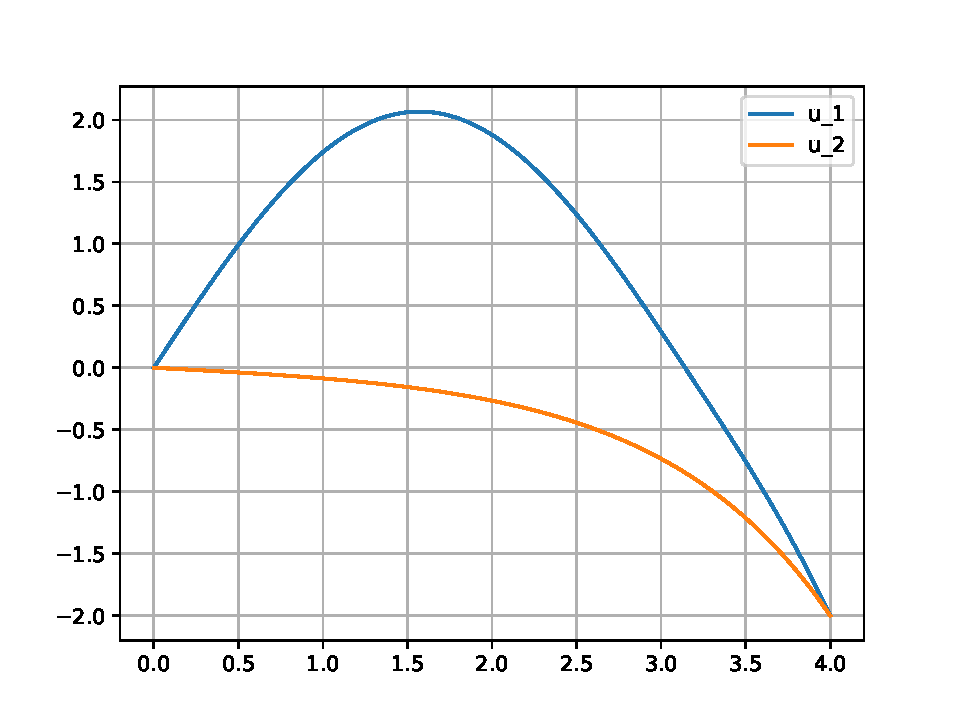
\includegraphics[width = 0.7\textwidth]{chapter_04/exercise_04_22_figure_3.pdf}
\end{center}





\subsection*{Version $u' = -|u|$}

Das gegebene Randwertproblem
\[
        u' = -|u(x)|,
  \quad u(0) =  0,
  \quad u(4) = -2
\]
für $u \in C^1[0,1]$ hat keine Lösung:

Die Funktion $u$ wäre monoton fallend, da $u'(x) = -|u(x)| \leq 0$ für alle $x \in [0,4]$ gilt.
Daher ist
\[
            I
  \coloneqq \{
              x \in [0,4]
            \mid
              u(x) < 0
            \}
\]
ein Intervall mit Randpunkt $4$.
Wegen der Stetigkeit von $u$ ist $I$ halboffen;
es gibt also $x_0 \in [0,4]$ mit $I = (x_0, 4]$.
Da $u(0) = 0$ gilt, ist dabei $x_0 > 0$.

Auf dem Intervall $I$ gilt nun $-|u| = u$.
Also erfüllt $u$ auf $I$ die Differenzialgleichung $u' = u$.
Somit gibt es eine Konstante $c \in \Real$ mit $u(x) = c e^x$ für alle $x \in I$.
Es gilt
\[
    -2
  = u(4)
  = c e^4
\]
und somit $c = -2 e^{-4}$.
Dann gilt aber
\[
    u(x_0)
  = \lim_{x \downarrow x_0} u(x)
  = \lim_{x \downarrow x_0} -2 e^{x-4}
  = -2 e^{x_0-4}
  < 0,
\]
im Widerspruch zu $x_0 \notin I$.

Unsere obige Argumentation spiegelt sich auch in dem Verhalten von \texttt{scipy} wieder:
Das folgende Programm würde eine Lösung der Differenzgliechung liefern und plotten:

\lstinputlisting[style=pythoncode, firstline = 1, lastline = 22]{chapter_04/exercise_04_22_old.py}

Wir erhalten den folgenden Graphen:

\begin{center}
  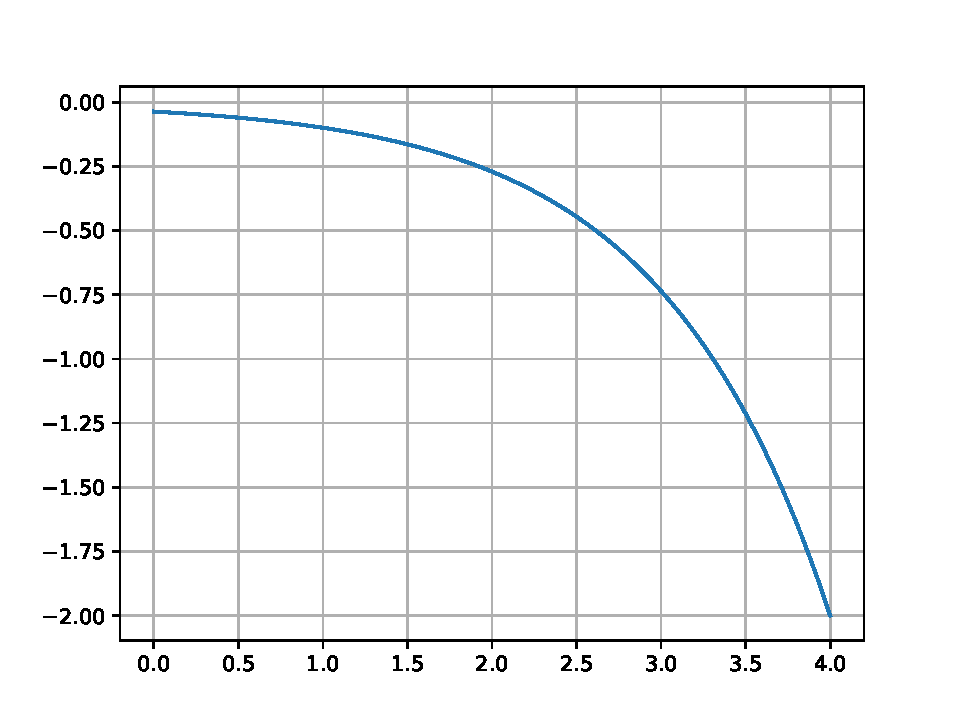
\includegraphics[width = 0.7\textwidth]{chapter_04/exercise_04_22_figure_1.pdf}
\end{center}

Die Randbedingung $u(4) = -2$ wird zwar beachtet, die Randbedingung $u(0) = 0$ hingegen nicht.
Der eingezeichnete Graph ist, wie auch aus der obigen Argumentation hervorgeht, der Graph von $-2 e^{x-4}$:

\begin{center}
  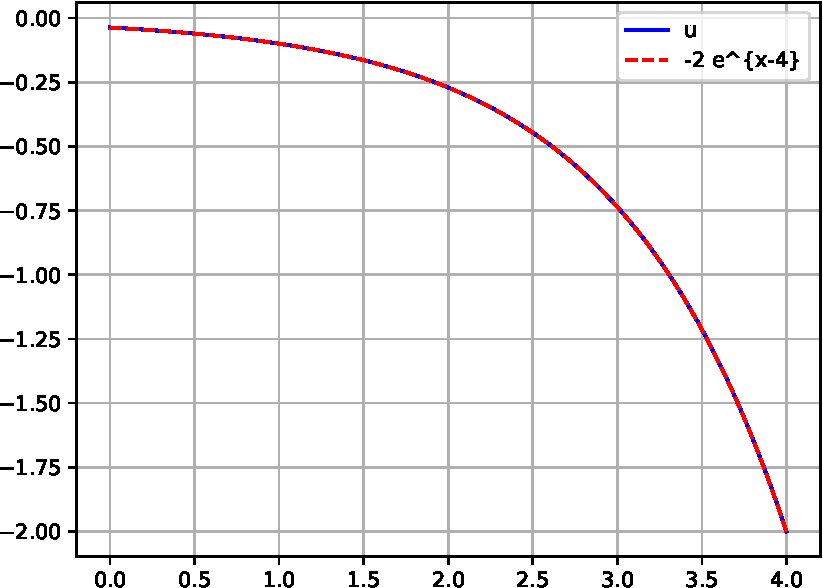
\includegraphics[width = 0.7\textwidth]{chapter_04/exercise_04_22_figure_2.pdf}
\end{center}














